\section{Přiklad 1}
% Jako parametr zadejte skupinu (A-H)
\prvniZadani{C}

\begin{figure}[!ht]
  \centering
  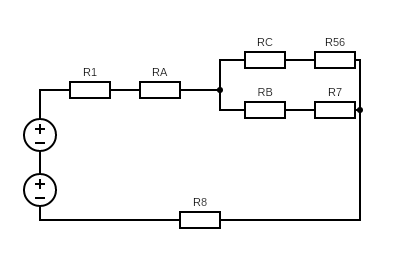
\includegraphics[width=0.9\textwidth, keepaspectratio]
  {/home/tjoslef/skola/zapisky/vut/IEL/projekt/sablona_reseni/fig/priklad1a.png}
  \caption{Uprava}
\end{figure}


\[
    R_{56} = \frac{R_6 \times R_5}{R_6 + R_5} \quad \Rightarrow \quad  R_{56} = 168.51063829787233
\]
\begin{figure}[!ht]
  \centering
  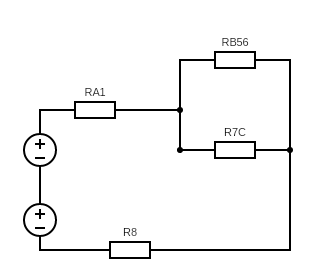
\includegraphics[width=0.7\textwidth, keepaspectratio]
  {/home/tjoslef/skola/zapisky/vut/IEL/projekt/sablona_reseni/fig/priklad1b.png}
  \caption{Další úprava}
\end{figure}




\[
R_{A1} = \frac{R_2 \cdot R_3}{R_2 + R_3 + R_4} + R_1 \quad \Rightarrow \quad R_{A1} = 576.1475409836065
\]
\[
    R_{B56} = \frac{R_2 \cdot R_4}{R_2 + R_3 + R_4} + \frac{R_6 \cdot R_5}{R_6 + R_5} \quad \Rightarrow \quad R_{B56} = 314.57621206836416
\]
\[
R_{C7} = \frac{R_3 \cdot R_4}{R_2 + R_3 + R_4} + R_7 \quad \Rightarrow \quad R_{C7} = 294.2622950819672
\]
\[
R = \left(\frac{R_{B56} \cdot R_{C7}}{R_{B56} + R_{C7}}\right) + R_{A1} + R_8 \quad \Rightarrow \quad R = 908.1877
\]
\[
I = \frac{U}{R} \quad \Rightarrow \quad I = 0.1982
\]
\[
    U_{B567C} = I \cdot \left( \frac{R_{B56} \cdot R_{C7}}{R_{B56} + R_{C7}} \right) \quad \Rightarrow \quad U_{B567C} = 30.13389439332759
\]
\[
    I_{C7} = \frac{U_{B567C}}{R_{C7}} \quad \Rightarrow \quad I_{C7} = 0.10240487788261746
\]
\[
    U_{R7} = I_{C7} \cdot R_7 \quad \Rightarrow \quad U_{R7} = 26.625268249480538
\]
\[
    U_{R3} = U - U_{R7} - U_{R1} - U_{R8} \quad \Rightarrow \quad U_{R_3} = 28.5107
\]
\[
    I_{R3} = \frac{U_{R3}}{R_3} \quad \Rightarrow \quad I_{R3} = 0.1501
\]



